\documentclass[12 pt]{report}

\usepackage{epsfig}
\usepackage[in,empty]{myfullpage}
\usepackage{amssymb}
\usepackage{amsmath}
\usepackage{tikz}

\unitlength = .5cm 

\baselineskip=20pt

\begin{document}

\noindent \vfill \noindent \large

\centerline{Math 324 C  - Summer 2016}

\centerline{Midterm exam 2}

\centerline{Wednesday, July 29th, 2016}

\normalsize

\vfill
\medskip
Name: \rule{10cm}{1pt}

\bigskip

\vfill
\begin{center}
{\large
\begin{tabular}{||c|c|r||}
\hline Problem 1 & 10 & \hspace{10mm} \hfill \\
\hline Problem 2 & 10  & \hspace{10mm} \hfill \\
\hline Problem 3 & 10 & \hspace{10mm} \hfill \\
\hline Problem 4 & 10  & \hspace{10mm} \hfill \\
\hline Problem 5 & 10  & \hspace{10mm} \hfill \\
\hline Total & 50 & \hspace{10mm} \hfill \\
\hline
\end{tabular}
}
\end{center}
\vfill
\begin{itemize}
\item There are 5 questions on this exam. Make sure you have all five.
\item You must show your work on all problems.  The correct answer
with no supporting work may result in no credit. \textbf{Put a box
around your FINAL ANSWER for each problem and cross out any work
that you don't want to be graded.} 
\item Give exact answers, and simplify as much as possible. 
For example, $\frac{\pi}{\sqrt{2}}$ is acceptable, but $3\sqrt{3}+\frac{1}{\sqrt{3}}$
should be reduced to $\frac{10\sqrt{3}}{3}$.   

\item If you need more room, use the backs
of the pages and indicate to the grader that you have done so.
\item Raise your hand if you have a question.
\item Any student found engaging in academic misconduct will receive
a score of 0 on this exam.
\item You have 60 minutes to complete the exam.  Budget your time wisely! \\
\end{itemize}
\vfill
\begin{center}GOOD LUCK!\end{center}

\newpage
\begin{enumerate}

\item (10 pts) Consider the function $f(x,y,z) = 3x \sin(y) - xz.$ 


\begin{enumerate} \item[a.] Find $\frac{\partial f}{\partial x}, \frac{\partial f}{\partial y}$ and $\frac{\partial f}{\partial z}$.

\item[b.] Let $v$ be the unit vector with tail at the origin and tip at the point $(1, \frac{\pi}{3}, \frac{\pi}{2})$ in spherical coordinates $(\rho, \theta, \phi)$. Find the directional derivative $D_vf$ at the point $(3, -\pi ,1)$. 

\item[c.] Give the unit vector $u$ that maximizes $D_uf(3,-\pi,1)$.  

\end{enumerate} 

\newpage 

\item[2a.] (3 pts) Give a definition in words of the tangent plane to a surface $F(x,y,z) = k$ at a point $p$ in terms of the gradient of $F$. (Don't just write down the equation.)  

\vspace{3cm} 

\item[2b.] (7 pts) Compute the tangent plane to the implicitly defined surface $x^2z+3y^3 -z^3- 3z = 0$ at the point $(x,y,z) = (1,1,1)$. 


\newpage

\item[3a.] (3 pts) Let $f(x,y) = \frac{1}{2}(x^2 + y^2)$. Write down a formula for $\nabla f(x,y)$, and draw the vector $\nabla f(x,y)$ at each of the three points $(1,0), (-2,1)$ and $(2,-2)$.  

\vspace{1cm}

\begin{picture}(10.5,10.5)(-5,-5)
  {\color{gray}
  \thinlines
  \multiput(-5,-4)(0,1){9}{\line(1,0){10}}
  \multiput(-4,-5)(1,0){9}{\line(0,1){10}}
  }
  \thicklines
  \put(-5,0){\vector(1,0){10.2}}
  \put(0,-5){\vector(0,1){10.2}}
  \put(5.3,0){\makebox(1,0)[l]{$x$}}
  \put(0,5.3){\makebox(0,1)[b]{$y$}}
\end{picture}

\vspace{1cm}

\item[3b.] (3 pts) Define what it means for a vector field $F$ defined on an \emph{arbitrary domain} $D$ in the plane to be conservative. (You may give any definition equivalent to the one we used in class.)

\vspace{4cm}

\item[3c.] (4 pts) Consider the vector field $F(x,y) = \langle y^3 \cos(x), - 3y^2 \sin(x) \rangle$. Is $F$ conservative? If so, give a potential function; if not, explain how you know it isn't conservative. 

\newpage

\item[4a.] (5 pts) State the fundamental theorem for line integrals, and use it to compute 

$$\int_C \sin(y) e^{x \sin(y)} dx + x \cos(y) e^{x \sin(y)} dy,$$

where $C$ is the line segment from $(1,\pi)$ to $(2,\pi)$ followed by the line segment from $(2,\pi)$ to $(2,2 \pi)$. 

\vspace{7cm}  

\item[4b.] (5 pts) Let $F$ denote the force field $F(x,y) = \langle 3 \ln (2xy-1), x^2-y^2 \rangle$ defined on $\{(x,y): 2xy > 1 \}$. Find the work done by $F$ on a particle traveling along the path $r(t) = (t, t^{-1}), 1 \leq t \leq 2$. 


\newpage

\item[5.] Consider the curve $C$ given by the equation $xy^2 = 1$ for $0 < x < \infty$. Let $D$ be the (infinite) region above $C$, so $D = \{(x,y): x > 0, y > \frac{1}{\sqrt{x}} \}$. Also, define the vector field $F$ by $F(x,y) = \langle \frac{1}{x^2+y^2}, \frac{1}{1+y^2} \rangle$. 

\item[5a.] (5 pts) Let $S_R$ be the quarter circle of radius $R$ centered at $(0,0)$ in the first quadrant parameterized counter-clockwise. By evaluating the line integral directly, show that

$$\lim_{R \to \infty} \int_{S_R} F \cdot dr = \frac{\pi}{2}.$$ 

\flushleft 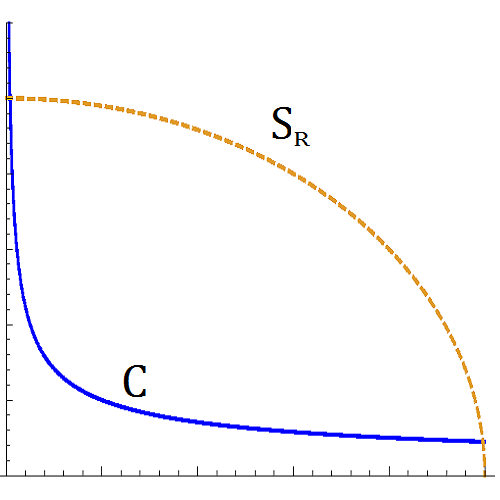
\includegraphics[width=2in]{midterm2s2016_problem_5.png}

\vspace{4cm} 

\item[5b.] (5 pts) Use the result from part a and Green's theorem to relate

$$\int_{C} F \cdot dr$$

to a double integral over the region $D$. (Hint: use Green's theorem on a closed curve consisting partly of $C$ and partly of $S_R$, and then let $R \to \infty$. You may assume that $C$ and $S_R$ meet at the points $(R,0)$ and $(0,R)$: the error in doing so is negligible.)

\newpage 


\item[5b.] (cont.)  

\vspace{8cm}
 
\item[5c.] (Extra credit) Evaluate your integral from part b: you may use the fact that 

$$\int \frac{x}{x^3+1} dx = \frac{1}{3} \log \frac{\sqrt{x^2-x+1}}{x+1} + \frac{1}{\sqrt{3}} \tan^{-1} \frac{2x-1}{\sqrt{3}} + C.$$ 

\end{enumerate}

\end{document}
